\documentclass{article}
% NeurIPS 2026 workshop submission: anonymous (default = submission mode with line numbers)
\usepackage{neurips_2026}
\makeatletter
\renewcommand{\@noticestring}{Submitted to the NeurIPS 2026 Workshop on Continual Learning in the Era of Foundation Models and Embodied Agents (CL4FMAgents). Do not distribute.}
\makeatother
\usepackage[utf8]{inputenc}
\usepackage[T1]{fontenc}
\renewcommand{\ttdefault}{lmtt}  % Type 1 typewriter; avoids the bitmap ectt (Type 3) font in \url
\usepackage{hyperref}
\hypersetup{colorlinks=true,linkcolor=blue!50!black,citecolor=blue!50!black,urlcolor=blue!50!black}
\usepackage{float}
\usepackage{url}
\usepackage{booktabs}
\usepackage{amsmath,amssymb,amsthm}
\usepackage{graphicx}
\usepackage{xcolor}
\usepackage{microtype}
\usepackage{enumitem}
\usepackage{algorithm}
\usepackage{algorithmic}
\usepackage{tikz}
\usetikzlibrary{arrows.meta,positioning,patterns,calc}
\graphicspath{{../figs/}}
\newcommand{\kwta}{$k$-WTA}
\newcommand{\pend}[1]{\textcolor{red}{#1}}  % numbers still being computed tonight; none may remain
\newtheorem{proposition}{Proposition}
\newtheorem{corollary}{Corollary}
\newtheorem{definition}{Definition}

\title{Replay in the Silent Degrees of Freedom: Continual Learning Without an Offline Phase}

\author{%
  Anonymous authors\\
  Paper under double-blind review
}

\begin{document}
\maketitle

\begin{abstract}
Replay-based continual learning rehearses past data either in an offline phase, during which
the agent stops acting, or interleaved with the live stream, where it perturbs the computation
serving the current input. An agent that learns in deployment can afford neither. Motivated by
local sleep, the use-dependent off-periods of individual cortical circuits in awake animals, we
show that replay can instead be written into the degrees of freedom the current input leaves
unused. In a network with $k$-winner-take-all hidden layers, confining replay updates to
synapses whose presynaptic unit is silent or whose postsynaptic unit is inactive leaves the
hidden computation on the current batch invariant: exactly so for silent and suppressed units,
and for all but $0.3\%$ of samples in practice. A refractory rule under which units that have
just fired sit out the next competition doubles the width of this channel and carries most of
the accuracy. On class-incremental split-MNIST the resulting learner, with no offline phase,
matches or exceeds the best offline rehearsal schedule, matches DER++, the strongest
interleaved-replay reference under backprop, and outperforms experience replay, ER-ACE and
unmasked interleaved replay; in a single pass over the stream, where one offline phase per
task is too few, it leads DER++ and its lead over offline rehearsal grows to $15$ points. On
split CIFAR-10 it again leads offline rehearsal and experience replay, but trails ER-ACE and
DER++ by two to three points. The construction is not tied to the local learner: on a
backprop network with $k$-winner-take-all hidden layers under the same schedule, refractory
rotation adds half a point in five epochs and three in a single pass, and isolation again
costs nothing on top of it.
\end{abstract}

% ================================================================ 1
\section{Introduction}
\label{sec:intro}

Foundation-model and embodied agents are increasingly expected to keep learning after
deployment, from streams that are non-stationary and never task-labelled. The dominant tool
against forgetting is replay from an episodic memory, and nearly every replay-based method
consumes it in one of two ways: in a dedicated offline phase, a ``night'' during which the
agent stops acting and rehearses, or by interleaving replayed samples with the live stream.
Both cost an agent. An offline phase is downtime during which the system is unavailable or
silently changing. Interleaved replay perturbs the computation currently serving the input.

Biology suggests a third option. Sleep-like off-periods occur \emph{locally}, in individual
cortical circuits of awake animals \citep{vyazovskiy2011}. Inducing such ON/OFF alternation in
one hemisphere of an awake mouse discharges local sleep pressure, inducing it bilaterally during
sleep deprivation rescues memory consolidation, and an equal tonic reduction of firing does not
discharge the pressure \citep{driessen2026}. Some core functions of sleep can thus be delivered
locally during wakefulness. We take this as an algorithmic motivation, not as a claim about
where biological consolidation occurs, and ask whether the computational degrees of freedom a
learner is not using can host consolidation while it acts, and what that costs.

We study the question in a deliberately constrained learner: a two-hidden-layer network with
sparse population codes, trained end to end by local rules with a single forward and feedback
sweep. Sparse codes expose exactly which degrees of freedom the current input does and does
not use, and local updates can be confined to them synapse by synapse. The contributions are:
\begin{itemize}[leftmargin=1.2em, itemsep=1pt, topsep=2pt]
\item \textbf{Isolated replay during inference.} A synapse may take a replay update only if
its presynaptic unit is silent for the current input or its postsynaptic unit is inactive.
Under \kwta{} dynamics this leaves the hidden computation on the current batch exactly
invariant for silent-presynaptic and suppressed units (Propositions~\ref{prop:pre}
and~\ref{prop:post}), and we measure how nearly it holds elsewhere.
\item \textbf{Refractory rotation.} Units that fired on the current batch sit out the next
competition. This alternation, the algorithmic counterpart of the ON/OFF requirement in
\citet{driessen2026}, doubles the consolidable channel and is the larger source of accuracy;
random and tonic controls locate what use-dependence and all-or-none silencing each add.
\item \textbf{Evaluation without an offline phase.} On class-incremental split-MNIST the
system matches offline rehearsal and DER++ and beats the other interleaved-replay references,
on the sequential stream and on the i.i.d.\ shuffle of the same data at once, at about twice
the offline schedule's replay samples; on split CIFAR-10 it keeps its lead over offline
rehearsal and experience replay but trails the cross-entropy backprop references. The
single-pass stream, the setting closest to an agent's, is where offline rehearsal fails and
the lead is largest. The same schedule on a backprop learner with \kwta{} hidden layers
shows that rotation and the isolation guarantee transfer beyond the local rule.
\end{itemize}
Every configuration is evaluated on two axes, the class-incremental stream and the identical
learner on the i.i.d.\ shuffle of the same data, because consolidation during inference must
not damage ordinary learning. The scale is small (MLPs on MNIST and CIFAR variants); the
object of study is the mechanism and its prerequisites (Section~\ref{sec:discussion}).

% ================================================================ 2
\section{Related work}
\label{sec:related}

\paragraph{Sleep-inspired consolidation.} The Bazhenov line implements sleep as a global
offline phase driven by noise under local plasticity \citep{tadros2022,bazhenov2026,golden2022,kubo2025};
wake--sleep frameworks with NREM/REM stages \citep{sorrenti2024,robinson2022} and systems such
as SIESTA \citep{harun2023} likewise schedule consolidation offline, and SESLR \citep{lin2026}
appends a noise-enhanced sleep phase to correct online learning's recency bias. None
consolidates in currently unused units during inference, and the bias correction such a phase
delivers is what our plastic readout receives continuously from isolated replay.

\paragraph{Gating and history-dependent competition.} Context-dependent gating activates a
subnetwork per task from task identity \citep{masse2018}; learned gates \citep{tilley2023},
dendritic context \citep{iyer2022}, task-free sparsification \citep{lassig2023} and recovered
functional masks \citep{mckee2026} derive the gate from the input. Refractory competition has
classical precedents \citep{kaski1994,maeda1999}, and spiking continual learners raise firing
thresholds with use \citep{shen2024} or randomise the top-$k$ selection \citep{shen2026} to
de-overlap task codes, the wake-side counterpart of our random-alternation control. Our
rotation differs in purpose: recently active units are benched for one competition to enlarge
a \emph{replay channel}, not to allocate resources across tasks.

\paragraph{Null-space and parameter isolation; replay baselines.} A mature line protects
\emph{previous} tasks: gradient or activation-subspace projections
\citep{farajtabar2020,saha2021,chaudhry2019}, feature-covariance null spaces
\citep{wangnscl2021}, $k$-winner sparsity with such projections \citep{abbasi2022}, frozen
subnetworks \citep{golkar2019,mallya2018}. We invert the protected direction: the ongoing
computation is held invariant while old-memory replay is written into degrees of freedom the
current sparse support exposes as invisible. No bases or task masks are stored, and the
``null space'' changes with every batch at no cost. Among interleaved-replay methods, DER++
\citep{buzzega2020} distils stored logits and ER-ACE \citep{caccia2022} restricts the incoming
loss to the classes present; both serve as references below. Complementary-learning-system
methods \citep{arani2022,pham2021} raise the value of each replayed sample but still replay at
every step, and learned replay scheduling \citep{klasson2023} is related to the trigger study
in Appendix~\ref{app:budget}.

% ================================================================ 3
\section{Method}
\label{sec:method}

\paragraph{Setting.} A stream of labelled examples is presented in $T$ contiguous tasks with
disjoint class sets; no task identity is available at test time; a single shared $C$-way
readout is evaluated on all classes after the last task (class-incremental learning). We
report final accuracy $A_{\mathrm{seq}}$, forgetting $F$, the accuracy $A_{\mathrm{iid}}$ of
the identical learner and budget on the i.i.d.\ shuffle (the \emph{static} axis), and the
replay cost $R$ in samples. The learner has an episodic memory of $K$ raw examples with
reservoir writing \citep{vitter1985}. The question is whether the offline term of
consolidation can be removed entirely without losing $A_{\mathrm{seq}}$, and at what price in
$A_{\mathrm{iid}}$ and $R$.

\paragraph{Base learner.} Layer activities are $a^0=x$ and, for $\ell=1,\dots,L$,
\begin{equation}
z^\ell = W^\ell a^{\ell-1} + b^\ell,\qquad
a^\ell = \Phi_k\!\big(\sigma(z^\ell)\odot(1-s^\ell)\big),
\label{eq:forward}
\end{equation}
where $\sigma$ is a rectifier, $s^\ell\in\{0,1\}^{n_\ell}$ the suppression mask of the
rotation rule below, and $\Phi_k$ keeps the $k$ largest entries of each row (\kwta). Layers
$1,\dots,L{-}1$ are hidden; layer $L$ is a linear $C$-way readout whose pre-activation $z^L$
is the output, scored by squared error against the one-hot target $y$. Errors come from one
top-down sweep through learned feedback weights $B^\ell\in\mathbb{R}^{n_{\ell+1}\times n_\ell}$
(no weight transport),
\begin{equation}
\varepsilon^L = y - z^L,\qquad
\varepsilon^\ell = \sigma'(z^\ell)\odot\Big((B^\ell)^{\!\top}\big[\kappa\tanh(\varepsilon^{\ell+1}/\kappa)\odot\mathbf{1}(a^{\ell+1}>0)\big]\Big),
\label{eq:sweep}
\end{equation}
a bounded, event-gated burst signal in the spirit of predictive-coding and burst-dependent
learners \citep{whittington2017,payeur2021}. Forward and feedback weights follow the same
local product with a shared decay $\lambda$ (Kolen--Pollack alignment
\citep{kolen1994,akrout2019}), $\Delta W^\ell\propto\varepsilon^\ell(a^{\ell-1})^{\!\top}-\lambda W^\ell$
and $\Delta B^{\ell-1}\propto\varepsilon^\ell(a^{\ell-1})^{\!\top}-\lambda B^{\ell-1}$, under
Dale's law with sign-concordant feedback and $30\%$ distance-dependent connectivity. The
optimiser is heavy-ball SGD with one per-synapse velocity; masked Adam ties it
(Appendix~\ref{app:further}). In development the whole constraint set cost about one point
against a dense backpropagation MLP on i.i.d.\ MNIST.

\paragraph{Isolated replay.} Let $X=\{x_b\}_{b=1}^{m}$ be the current waking batch,
$a^\ell_{i,b}$ the activity of unit $i$ on sample $b$, and
$\mathcal{A}^\ell(X)=\{i:\exists b,\ a^\ell_{i,b}\neq0\}$ the awake set. During the same
forward step, a replay micro-batch drawn from the buffer is applied through the synapse mask
\begin{equation}
M^\ell_{ij}=\mathbf{1}\big[\,j\notin\mathcal{A}^{\ell-1}(X)\ \lor\ i\notin\mathcal{A}^\ell(X)\,\big],
\label{eq:mask}
\end{equation}
i.e.\ iff the presynaptic unit is silent for the current input or the postsynaptic unit is
asleep. The mask applies to the \emph{entire} replay-induced parameter change, not only to the
data gradient: with heavy-ball velocity $v$ ($\mu=0.9$), the local update direction
$G=\varepsilon^\ell(a^{\ell-1})^{\!\top}$ and the per-step decay coefficient $\lambda$, a
replay step is
\begin{equation}
v\leftarrow M\odot(\mu v+G)+(1-M)\odot v,\qquad
W\leftarrow W+\eta\,M\odot v-\lambda\,M\odot W,
\label{eq:maskedstep}
\end{equation}
so the velocity is frozen (not zeroed) outside the mask, the decay is confined to it, and
biases follow the unit mask $\mathbf{1}[i\notin\mathcal{A}^\ell(X)]$; unmasked momentum would
re-inject the update into awake synapses \citep{mckee2026,bricken2023}. The readout row and
its bias stay plastic, so old classes remain calibrated; the guarantees below concern the
hidden computation. Within one step the order is: forward pass under the current suppression,
unmasked waking update, awake sets from that pass, masked replay on the updated weights;
replay is inferred with the suppression removed, so a refractory unit may fire on replay and
learn from it (Algorithm~\ref{alg:step}).

\begin{algorithm}[t]
\caption{One waking step of the default system (rotation always on, one micro-batch per batch).}
\label{alg:step}
\begin{algorithmic}[1]
\REQUIRE weights $W_t$, velocities $v_t$, suppression $s(t)$, buffer $\mathcal{M}$
\STATE $a\leftarrow\mathrm{forward}(X_t;\,W_t,\,s(t))$,\ \ $\varepsilon\leftarrow\mathrm{sweep}(a,y_t)$ \hfill Eqs.~\eqref{eq:forward}--\eqref{eq:sweep}
\STATE $(W,v)\leftarrow$ unmasked heavy-ball step on $(W_t,v_t)$ with $G^\ell=\varepsilon^\ell(a^{\ell-1})^{\!\top}$, rate $\eta_w$ \hfill wake update
\STATE $\mathcal{A}^\ell\leftarrow\{i:\exists b,\ a^\ell_{i,b}\neq0\}$ for every hidden layer \hfill from the pre-update $a$
\STATE $M^\ell\leftarrow$ Eq.~\eqref{eq:mask}, unit mask $\mathbf{1}[i\notin\mathcal{A}^\ell]$, readout row and bias unmasked
\STATE $s^\ell_i(t{+}1)\leftarrow\mathbf{1}[i\in\mathcal{A}^\ell]$ \hfill refractory rotation
\STATE write $(X_t,y_t)$ into $\mathcal{M}$ (reservoir)
\STATE $(X_r,y_r)\sim\mathcal{M}$;\ \ $a_r\leftarrow\mathrm{forward}(X_r;\,W,\,s{=}0)$,\ \ $\varepsilon_r\leftarrow\mathrm{sweep}(a_r,y_r)$ \hfill suppression removed
\STATE $(W,v)\leftarrow$ masked step, Eq.~\eqref{eq:maskedstep}, with $G^\ell=\varepsilon^\ell_r(a^{\ell-1}_r)^{\!\top}$, rate $\eta_r$, masks $M^\ell$
\RETURN $W_{t+1}=W$,\ $v_{t+1}=v$,\ $s(t{+}1)$
\end{algorithmic}
\end{algorithm}

\begin{proposition}[Pre-silent updates are exactly invisible]\label{prop:pre}
Fix $X$ and let $\widehat W^\ell=W^\ell+\Delta^\ell$ with $\Delta^\ell_{ij}=0$ whenever
$j\in\mathcal{A}^{\ell-1}(X)$. Then every hidden activity on every sample of $X$ is
unchanged for any magnitude of $\Delta$; if the readout row satisfies the same condition, or
is held fixed, the network output is unchanged as well.
\end{proposition}
\begin{proposition}[Post-asleep updates are invisible under a margin]\label{prop:post}
Let $\Delta^\ell$ and $\Delta b^\ell$ additionally move synapses and biases of units
$i\notin\mathcal{A}^\ell(X)$ with active presynaptic partners, and write
$\delta_{i,b}=\sum_j\Delta^\ell_{ij}a^{\ell-1}_{j,b}+\Delta b^\ell_i$. If for every such unit
and every sample $\sigma(z^\ell_{i,b}+\delta_{i,b})<\tau^\ell_{k,b}$, where $\tau^\ell_{k,b}$
is the $k$-th largest value entering $\Phi_k$ on sample $b$ (strict, so a tie cannot promote
the unit; when fewer than $k$ entries are positive, $\tau^\ell_{k,b}=0$ and the condition
reads $\sigma(\cdot)=0$), the hidden activities on $X$ are unchanged.
\end{proposition}
\begin{corollary}[Suppressed units are exact for any magnitude]\label{cor:refr}
If $s^\ell_i=1$ in \eqref{eq:forward}, $a^\ell_{i,b}=0$ for every sample and
Proposition~\ref{prop:post} holds with no margin condition.
\end{corollary}
Proofs are in Appendix~\ref{app:proofs}. The propositions take the mask and the weights it
protects from the same state; in the implemented order the awake sets precede the waking
update, so they hold exactly for the pre-update weights and the one-step lag is part of the
measured drift. The default system does not enforce the margin, so we measured it over all
$16{,}885$ isolated replay updates of the reported run (three seeds): the update altered the
top hidden code of $0.33\%$ of waking samples ($0.31$--$0.35$) and a waking prediction for
$0.32\%$, almost all through the plastic readout ($0.001\%$ with the readout isolated), and
violated the margin for $\sim\!10^{-4}$ of asleep units per step. The isolation is thus exact
for silent-presynaptic and suppressed units and near-exact elsewhere for the hidden code of
the \emph{current} batch. What replay does to later inputs is measured by the ablation, and
Corollary~\ref{cor:refr} is why rotation makes the isolation robust.

\paragraph{Refractory rotation.} After batch $X_t$, set
$s^\ell_i(t{+}1)=\mathbf{1}[i\in\mathcal{A}^\ell(X_t)]$: every unit that fired sits out the
next competition and is therefore asleep, and exactly consolidable, for $X_{t+1}$. Rotation
widens the isolated channel
$\rho_\ell=|\tilde{\mathcal{A}}^\ell\setminus\mathcal{A}^\ell(X)|/|\tilde{\mathcal{A}}^\ell|$,
the fraction of the units $\tilde{\mathcal{A}}^\ell$ activated by the replay micro-batch that
are asleep for the current input, from $0.2$--$0.3$ to $\approx0.53$, at the price of running
inference on the second-best coalition of units (Figure~\ref{fig:mech}). The default system
runs rotation on every batch and one replay micro-batch beside every waking batch; internal
triggers that schedule sparse replay budgets, and a novelty gate on rotation, are described
in Appendix~\ref{app:budget} and are not needed for the results below.

\begin{figure}[t]
\centering
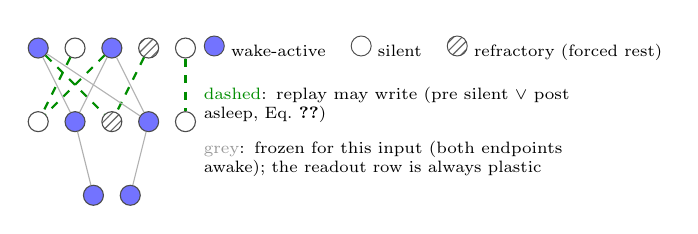
\begin{tikzpicture}[
  scale=0.85, transform shape,
  font=\scriptsize, >=Latex,
  unit/.style={circle, draw=black!70, minimum size=8.5pt, inner sep=0pt},
  awake/.style={unit, fill=blue!55},
  asleep/.style={unit, fill=white},
  refr/.style={unit, pattern=north east lines, pattern color=black!60},
]
\foreach \i/\st in {0/awake,1/asleep,2/awake,3/refr,4/asleep}
  \node[\st] (x\i) at (0.55*\i, 2.2) {};
\foreach \i/\st in {0/asleep,1/awake,2/refr,3/awake,4/asleep}
  \node[\st] (h\i) at (0.55*\i, 1.1) {};
\node[awake] (o0) at (0.825, 0.0) {};
\node[awake] (o1) at (1.375, 0.0) {};
\draw[green!55!black, dashed, thick] (x1) -- (h0);
\draw[green!55!black, dashed, thick] (x3) -- (h2);
\draw[green!55!black, dashed, thick] (x4) -- (h4);
\draw[green!55!black, dashed, thick] (x2) -- (h0);
\draw[green!55!black, dashed, thick] (x0) -- (h2);
\draw[black!30] (x0) -- (h1); \draw[black!30] (x2) -- (h1);
\draw[black!30] (x0) -- (h3); \draw[black!30] (x2) -- (h3);
\draw[black!30] (h1) -- (o0); \draw[black!30] (h3) -- (o1);
\node[align=left, anchor=west] at (2.35, 2.2)
  {\tikz\node[awake]{}; wake-active \quad \tikz\node[asleep]{}; silent \quad \tikz\node[refr]{}; refractory (forced rest)};
\node[align=left, anchor=west, text width=6.2cm] at (2.35, 1.35)
  {\textcolor{green!55!black}{dashed}: replay may write (pre silent $\lor$ post asleep, Eq.~\ref{eq:mask})};
\node[align=left, anchor=west, text width=6.2cm] at (2.35, 0.55)
  {\textcolor{black!40}{grey}: frozen for this input (both endpoints awake); the readout row is always plastic};
\end{tikzpicture}
\caption{\textbf{Isolated replay with refractory rotation.} During each waking batch, replay
from the episodic buffer is written only into hidden synapses invisible to the current input,
exactly so for silent presynaptic and suppressed units; refractory rotation forces the units
that just fired into the consolidable set for the next batch.}
\label{fig:mech}
\end{figure}

\paragraph{Protocol.} Split-MNIST (five tasks of two classes) and split CIFAR-10 (same
protocol, $32{\times}32$ luminance), each with five epochs per task and, as the single-pass
protocol, one epoch per task; each with its i.i.d.\ counterpart. Architecture
$d$--$512$--$256$--$C$, \kwta{} $10\%$, waking batches of $16$, one replay micro-batch of
$16$ per waking batch, buffer $K{=}1000$. Baselines: the offline ``night'' on the same
learner ($20$ replay batches of $256$ at $3\times$ learning rate after each waking epoch, the
best offline schedule in our sweep) and on its preferred narrower core; interleaved replay for
the local learner without the mask; and, under backprop with the same buffer, experience
replay (BP+ER), DER++ \citep{buzzega2020}, ER-ACE \citep{caccia2022} and A-GEM
\citep{chaudhry2019}, each at its best width and loss. To test the mechanism off the local
learner, the same schedule also runs on a backprop MLP of the same width with \kwta{} hidden
layers (Table~\ref{tab:bpk}), with Adam's moments confined to the mask as the velocity is
here and its learning rate selected on the development split. Six seeds on the reported
split and three on the second, mean $\pm$ s.d. Configurations were selected on the official
test splits, which served as the development set, and then frozen; every number reported in
the main text re-trains the frozen configuration with a stratified tenth of the training data
removed from the stream and evaluates on that tenth, which took part in no selection (during
development it was part of the training stream and never evaluated on). A second tenth drawn
with a different seed replicates the headline rows (Appendix~\ref{app:val}). Forgetting $F$
is the mean drop of each earlier task's accuracy from its own end to the end of training.
Evaluation runs with the suppression mask off (\kwta{} only), so test order and batch size
cannot affect it. Details of the sweeps and of the cost accounting are in
Appendix~\ref{app:cost}.

% ================================================================ 4
\section{Results}
\label{sec:results}

\begin{table}[t]
\centering\footnotesize
\caption{\textbf{Split-MNIST, class-incremental, $K{=}1000$} (held-out split). Sequential:
five epochs per task; i.i.d.: the same learner on the shuffled stream; single pass: one epoch
per task. Mean $\pm$ s.d.\ over six seeds.}
\label{tab:ablation}
\begin{tabular}{@{}lccc@{}}
\toprule
Variant & Sequential & i.i.d. & Single pass \\
\midrule
\textbf{isolated replay $+$ rotation (ours)} & $\mathbf{91.6\pm0.3}$ & $94.1\pm0.2$ & $\mathbf{91.8\pm0.3}$ \\
\quad $-$ rotation (isolated replay on natural silence) & $88.0\pm0.7$ & $95.4\pm0.2$ & $86.4\pm1.0$ \\
\quad $-$ isolation (rotation, unmasked replay) & $91.5\pm0.3$ & $93.7\pm0.3$ & $91.5\pm0.8$ \\
\quad $-$ both (unmasked interleaved replay) & $85.4\pm3.5$ & $93.8\pm5.0$ & $83.0\pm14.9$ \\
\quad random rotation of matched size & $91.1\pm0.7$ & $92.3\pm0.3$ & $90.5\pm0.9$ \\
\quad replay confined to the readout & $41.7\pm10.9$ & $81.2\pm2.5$ & $25.1\pm3.0$ \\
\quad mirror isolation (protect the past instead) & $79.4\pm3.5$ & $90.2\pm3.0$ & $80.9\pm4.1$ \\
\quad soft rotation (gain $0.5$ instead of $0$) & $89.9\pm0.7$ & $84.6\pm0.8$ & $87.8\pm1.4$ \\
\quad no replay & $19.4\pm0.0$ & $95.1\pm0.1$ & $18.1\pm0.5$ \\
\midrule
offline rehearsal, same learner & $89.0\pm3.5$ & --- & $76.9\pm3.4$ \\
offline rehearsal, narrow learner & $88.5\pm2.8$ & --- & $71.5\pm1.9$ \\
\midrule
BP $+$ ER & $88.8\pm0.3$ & $97.4\pm0.1$ & $88.6\pm0.2$ \\
BP $+$ DER++ & $91.5\pm0.5$ & --- & $90.1\pm0.7$ \\
BP $+$ ER-ACE & $90.2\pm0.4$ & --- & $88.5\pm0.3$ \\
BP $+$ A-GEM & $68.5\pm7.0$ & --- & $46.8\pm5.0$ \\
\bottomrule
\end{tabular}
\end{table}

\paragraph{Consolidation without an offline phase.} Table~\ref{tab:ablation} is the
main result. With one isolated replay micro-batch beside every waking batch and no offline
phase, the system reaches $91.6\pm0.3\%$ on split-MNIST. Offline rehearsal on the same
learner, the reference that does have downtime, reaches $89.0\pm3.5$ on this split with a
bimodal spread across seeds, and $91.5\pm0.5$ on the second held-out split; the narrower
learner it prefers reaches $88.5\pm2.8$ and $89.3\pm0.6$. Consolidation during inference thus
matches the offline reference on both splits and exceeds it on the first. Against the methods
that, like ours, have no offline phase, the lead is consistent: $+2.8$ points over BP+ER
(seed-paired, $95\%$ interval $[+2.5,+3.2]$), $+6.3$ over unmasked interleaved replay on our
own learner, $+1.5$ over ER-ACE and $+23$ over A-GEM, whose gradient projection protects the
past at the expense of the present. DER++, which distils stored logits, is the one reference
the system does not beat: the two tie at $91.5\pm0.5$ and $91.6\pm0.3$, a paired difference
of $0.1$ $[-0.3,+0.4]$. In a single pass over the stream the picture sharpens: the system loses
nothing ($91.8\pm0.3$), DER++ drops to $90.1\pm0.7$ and BP+ER holds at $88.6$, unmasked
replay becomes unstable ($83.0\pm14.9$), and offline rehearsal falls to $76.9\pm3.4$ because
one night per task is too few. The price on the static axis is $1.0$ point against the same
learner without replay ($95.1$) and $3.3$ against dense backprop.

\paragraph{What rotation and isolation each buy.} Removing rotation costs $3.6$ sequential
points ($88.0\pm0.7$, the same mask on natural silence alone) and removing both rotation and
isolation $6.2$, with a twelve-fold larger seed deviation. Removing isolation alone costs
nothing measurable in mean accuracy: rotation with unmasked replay reaches $91.5\pm0.3$, a
seed-paired margin of $0.1$ $[-0.3,+0.5]$, and $0.4$ points on the static axis. The factors
are therefore strongly sub-additive, rotation being the larger. Figure~\ref{fig:batch} (left)
varies the replay batch size with the number of updates fixed. The full system is flat from $256$
down to $8$ samples ($91.6\to91.1$) and loses $1.9$ at $4$, where unmasked replay without
rotation ($85.4\pm3.5$ at $16$) and the offline night ($85.8\pm3.0$ at $16$) have already
degraded. Rotation with unmasked replay tracks the full system to within seed noise down to
batch $4$. At two-sample batches both lose heavily, but isolated replay degrades gracefully
($79.0\pm3.2$, every seed within $75$--$84$) where unmasked replay fails severely, below
$60\%$, in three of six seeds (Appendix~\ref{app:isomargin}). In the seeds and configurations
tested, isolation's contribution to accuracy is the absence of those failures; what it buys
at every batch size is the guarantee on the live computation, without which the outcome
rests on the rotation's tolerance of the perturbation.

\begin{figure}[t]
\centering
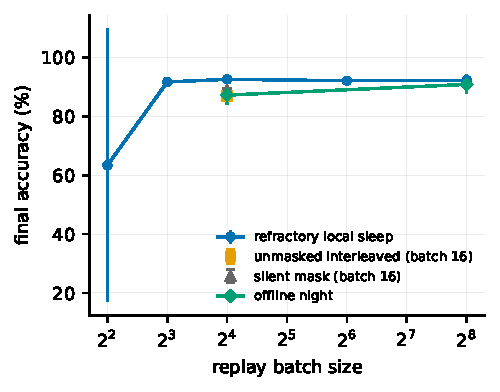
\includegraphics[width=.40\linewidth]{fig_batch.pdf}\hfill
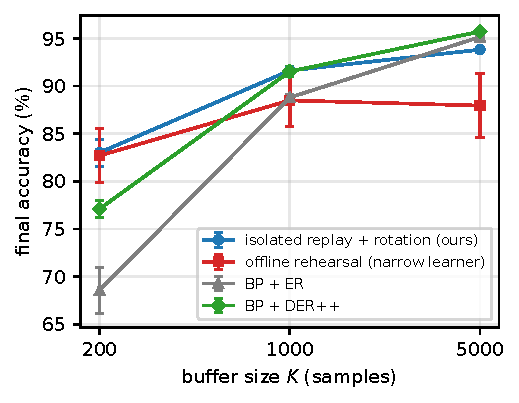
\includegraphics[width=.40\linewidth]{fig_ksweep.pdf}
\caption{\textbf{Left (replay batch size):} split-MNIST accuracy against the replay batch
size, the number of updates fixed within each series (one per waking batch; $20$ per epoch
for the night, whose samples therefore fall with its batch): the full system is flat down to
$8$ samples and loses $1.9$ at $4$ ($12.7$ at $2$, Appendix~\ref{app:isomargin}); rotation
with unmasked replay (dashed) trails it by $0.1$ to $0.3$, within seed noise, and fails
severely in half the seeds at batch $2$; without rotation, unmasked and isolated replay and
the offline night all degrade. \textbf{Right (buffer size):} accuracy against the buffer size
$K$ for the system and the replay references (held-out split, six seeds).}
\label{fig:batch}
\end{figure}

\paragraph{Controls.} Replay confined to the readout row falls to $41.7\pm10.9$ and costs
$13$ static points, so hidden-layer replay updates are essential. A random suppression of
matched size recovers most of rotation's gain ($91.1\pm0.7$) but trails it by $0.5$
sequential and $1.8$ static points with $1.3\times$ the forgetting: alternating the coalition
carries most of the effect, and resting the recent winners the rest. Soft rotation, halving
rather than silencing the recent winners, loses on both axes ($89.9/84.6$), so all-or-none
OFF periods beat turned-down gain, as in the biological tonic control. Mirror isolation,
which bars the waking update from the synapses that served the last replay batch and leaves
replay unmasked, reaches $79.4\pm3.5$; this reversed mask is one implementation of the
protect-the-past direction and loses twelve points, which locates the value in the direction
of protection and not in masking as such. The unmasked control is not handicapped
by its replay step: over replay gains $\{1/16,1/4,1,3,10\}$ it plateaus from gain $1$ to $3$
($85.7$, $85.4$) and never closes the gap (Appendix~\ref{app:further}).

\paragraph{Transfer to CIFAR-10.} On raw split CIFAR-10 (Table~\ref{tab:cifar}) the ordering
among the local-learner variants and BP+ER transfers and widens: isolated replay with rotation
$28.4\pm0.8$, offline rehearsal $25.1\pm2.7$, BP+ER $24.6\pm0.6$, and unmasked interleaved
replay $14.6\pm4.6$, no better than no replay at all ($16.3$); the second held-out split gives
$29.7>26.5>25.8>15.5$. The two cross-entropy references under backprop lead here: ER-ACE by
$3.2$ points and DER++ by $2.2$ (seed-paired, $[+2.1,+4.4]$ and $[+1.1,+3.2]$), and in a
single pass ER-ACE keeps its lead ($29.5$ against $26.0$) while DER++ falls behind
($24.4\pm1.2$). All methods are far from the i.i.d.\ ceiling on this input, so CIFAR-10 tests
orderings rather than levels, and two survive it: removing the offline phase costs nothing
against offline rehearsal, and against the best backprop references it is the local learner
itself, not the consolidation mechanism, that falls short.

\begin{table}[t]
\centering\footnotesize
\caption{\textbf{Raw split CIFAR-10, class-incremental, $K{=}1000$}. Sequential accuracy on
the reported held-out split (six seeds), on a second held-out split (three seeds), and in a
single pass (six seeds).}
\label{tab:cifar}
\begin{tabular}{@{}lccc@{}}
\toprule
Method & Sequential & Second split & Single pass \\
\midrule
\textbf{isolated replay $+$ rotation (ours)} & $28.4\pm0.8$ & $29.7\pm0.9$ & $26.0\pm1.9$ \\
offline rehearsal, same learner & $25.1\pm2.7$ & $26.5\pm0.4$ & $21.6\pm1.0$ \\
unmasked interleaved replay & $14.6\pm4.6$ & $15.5\pm4.5$ & $14.5\pm3.9$ \\
no replay & $16.3\pm0.1$ & $16.6\pm0.0$ & $11.7\pm1.1$ \\
BP $+$ ER & $24.6\pm0.6$ & $25.8\pm0.8$ & $25.8\pm0.7$ \\
BP $+$ DER++ & $30.7\pm0.8$ & $31.0\pm0.6$ & $24.4\pm1.2$ \\
BP $+$ ER-ACE & $\mathbf{31.6\pm1.0}$ & $\mathbf{31.7\pm0.8}$ & $\mathbf{29.5\pm0.8}$ \\
BP $+$ A-GEM & $16.5\pm0.2$ & $16.7\pm0.2$ & $15.3\pm0.3$ \\
\bottomrule
\end{tabular}
\end{table}

\paragraph{Cost.} Samples are not the only cost. The headline schedule replays
$2.2\times$ the night's samples ($2.7\times10^5$ against $1.2\times10^5$) in $35\times$ as
many updates ($16{,}885$ masked micro-batch updates against $480$ night batches). Two
schedules meet the night's budget within $1.1\times$ and keep the accuracy: eight-sample
micro-batches at every waking batch ($91.1\pm0.4$) and $16$-sample ones at every second
batch ($91.2\pm0.2$). Accuracy therefore depends on the frequency of small isolated updates
rather than on the number of replayed samples. In wall-clock on one CPU thread the headline
run takes $8.8$ minutes against $1.4$ for the night, $8.6$ for unmasked interleaved replay and
$1.0$ with no replay, in an unoptimised implementation whose mask construction is dense: the
per-batch replay step, not the sample count, is the online price of consolidating during the
stream (Appendix~\ref{app:cost}).

\paragraph{Buffer size.} Figure~\ref{fig:batch} (right) varies the buffer. At $K{=}200$ the
system leads every reference ($83.0\pm1.4$ against $82.7\pm2.9$ for offline rehearsal,
$77.1\pm0.9$ for DER++ and $68.5\pm2.4$ for BP+ER); at $K{=}1000$ it ties DER++; at
$K{=}5000$ the backprop references pull ahead ($95.7$ for DER++ and $95.2$ for BP+ER
against $93.8\pm0.2$), while offline rehearsal on the local learner saturates near $88$. The
mechanism's advantage is therefore largest where an agent's memory is smallest, and at large
buffers the ceiling is the local learner's own i.i.d.\ accuracy ($94.1$), not the mechanism.

\paragraph{The mechanism on a backprop learner.} Nothing in the construction requires the
local rule, so Table~\ref{tab:bpk} runs the same schedule on a backprop MLP of the same width
with \kwta{} hidden layers at the same $10\%$ fraction. Rotation transfers: it lifts
interleaved replay from $91.7\pm0.4$ to $92.2\pm0.3$ (seed-paired $+0.5$ $[+0.2,+0.8]$) and
from $89.3$ to $92.7$ in a single pass ($+3.4$ $[+2.8,+4.0]$), to the level of the local
learner and of DER++ under its own batch-$256$ protocol ($91.5$), at a static price of
$0.5$--$0.9$ points. Isolation on top of rotation
again costs nothing ($-0.1$ $[-0.3,+0.1]$) and brings the guarantee. Isolation alone,
however, hurts the backprop learner ($84.7\pm2.6$, seven points below interleaved replay)
where it helped the local one: without rotation the channel that natural silence leaves open
is too narrow for this learner, so on backprop the guarantee is affordable only through the
rotation. The schedule itself is also worth three points to backprop (interleaved replay in
$16$-sample micro-batches reaches $91.7$ against $88.8$ for BP+ER in batches of $256$).

\begin{table}[t]
\centering\footnotesize
\caption{\textbf{The same schedule on a backprop learner} ($512$--$256$, \kwta{} $10\%$, Adam,
waking batches of $16$ with one $16$-sample replay micro-batch each, $K{=}1000$; held-out
split, six seeds; learning rate selected on the development split).}
\label{tab:bpk}
\begin{tabular}{@{}lccc@{}}
\toprule
BP $+$ \kwta{} & Sequential & i.i.d. & Single pass \\
\midrule
interleaved replay (unmasked) & $91.7\pm0.4$ & $97.2\pm0.1$ & $89.3\pm0.6$ \\
isolated replay & $84.7\pm2.6$ & $97.6\pm0.1$ & $81.9\pm2.1$ \\
interleaved replay $+$ rotation & $\mathbf{92.2\pm0.3}$ & $96.7\pm0.3$ & $92.7\pm0.3$ \\
isolated replay $+$ rotation & $92.1\pm0.3$ & $96.6\pm0.1$ & $\mathbf{92.8\pm0.2}$ \\
\bottomrule
\end{tabular}
\end{table}

% ================================================================ 5
\section{Discussion}
\label{sec:discussion}

\paragraph{What this offers agents.} The construction is a recipe with two prerequisites,
both of which can be checked on a given architecture. The representation must be sparse
enough that a batch leaves most hidden units silent, and the replay update must be maskable
synapse by synapse. Nothing in Propositions~\ref{prop:pre} and~\ref{prop:post} depends on how
the update is computed; we studied a local learner because its sparse codes and local rules
make both prerequisites hold by construction, and Table~\ref{tab:bpk} shows the same
schedule on a backprop learner with \kwta{} layers: rotation transfers, isolation costs
nothing on top of it, and isolation alone does not transfer. Top-$k$ routed
mixture-of-experts layers expose, per token, the experts a token leaves silent; whether the
routes of a whole batch leave enough experts idle is a measurement, since load balancing
pushes against it. Under these prerequisites, consolidation can run in the silent degrees of
freedom between the steps of the stream, with no separate offline phase, under a conditional
guarantee on the computation in use, at a higher total compute ($6\times$ the night's
wall-clock, unoptimised). We treat the biology as analogy, not as mechanistic equivalence;
the refractory rule mirrors the ON/OFF finding of \citet{driessen2026}, and the dissociation
of triggers in Appendix~\ref{app:budget} is a testable prediction.

\paragraph{Limitations.} All results are at MLP scale on MNIST and CIFAR-10, with six seeds
on held-out training data and three on a second held-out split. The lead over the
best offline night is $2.6$ points on the first split and $0.3$ on the second, where the
night's seed variance vanished; the leads over the interleaved-replay references hold on
both. DER++ ties the system on split-MNIST and trails it only in the single pass, and on raw
CIFAR-10 ER-ACE and DER++ lead it by two to three points, so the comparison with interleaved
replay is not a claim of a new accuracy level; the contribution is consolidation with the live
computation held invariant, at no loss on split-MNIST against the strongest such reference.
Rotation keeps a static price of $1$--$2$ points at this activity fraction. The rule's synaptic decay is tuned once per dataset; a
drive-referenced controller that replaces it by one ratio target and, with locally learned
skip synapses, holds a five-hidden-layer network at the two-layer level is reported in
Appendix~\ref{app:controller}. Code can be found at
\url{https://anonymous.4open.science/r/IaC-CL-with-no-offline}

\clearpage
\bibliographystyle{plainnat}
\begin{thebibliography}{99}\small

\bibitem[Abbasi et al.(2022)]{abbasi2022} Abbasi, A., Nooralinejad, P., Braverman, V., Pirsiavash, H., Kolouri, S. (2022). Sparsity and heterogeneous dropout for continual learning in the null space of neural activations. In \emph{Conference on Lifelong Learning Agents (CoLLAs)}, PMLR 199.

\bibitem[Akrout et al.(2019)]{akrout2019} Akrout, M., Wilson, C., Humphreys, P., Lillicrap, T., Tweed, D. (2019). Deep learning without weight transport. In \emph{NeurIPS} 32.

\bibitem[Arani et al.(2022)]{arani2022} Arani, E., Sarfraz, F., Zonooz, B. (2022). Learning fast, learning slow: A general continual learning method based on complementary learning system. In \emph{ICLR}.

\bibitem[Bazhenov et al.(2026)]{bazhenov2026} Bazhenov, A., Delanois, J.E., Krishnan, G.P. (2026). Not just after one: Sleep-inspired replay prevents catastrophic forgetting after sequential tasks. \emph{arXiv:2606.08447}.

\bibitem[Borb\'ely(1982)]{borbely1982} Borb\'ely, A.A. (1982). A two process model of sleep regulation. \emph{Human Neurobiology}, 1:195--204.

\bibitem[Bricken et al.(2023)]{bricken2023} Bricken, T., Davies, X., Singh, D., Krotov, D., Kreiman, G. (2023). Sparse distributed memory is a continual learner. In \emph{ICLR}.

\bibitem[Buzzega et al.(2020)]{buzzega2020} Buzzega, P., Boschini, M., Porrello, A., Abati, D., Calderara, S. (2020). Dark experience for general continual learning: A strong, simple baseline. In \emph{NeurIPS} 33.

\bibitem[Caccia et al.(2022)]{caccia2022} Caccia, L., Aljundi, R., Asadi, N., Tuytelaars, T., Pineau, J., Belilovsky, E. (2022). New insights on reducing abrupt representation change in online continual learning. In \emph{ICLR}.

\bibitem[Chaudhry et al.(2019)]{chaudhry2019} Chaudhry, A., Ranzato, M., Rohrbach, M., Elhoseiny, M. (2019). Efficient lifelong learning with A-GEM. In \emph{ICLR}.

\bibitem[Driessen et al.(2026)]{driessen2026} Driessen, K., Squarcio, F., Tononi, G., Cirelli, C. (2026). Induction of cortical ON/OFF periods in awake mice fulfills sleep functions. \emph{Nature Neuroscience}, 29:1954--1965.

\bibitem[Farajtabar et al.(2020)]{farajtabar2020} Farajtabar, M., Azizan, N., Mott, A., Li, A. (2020). Orthogonal gradient descent for continual learning. In \emph{AISTATS}, PMLR 108.

\bibitem[Golden et al.(2022)]{golden2022} Golden, R., Delanois, J.E., Sanda, P., Bazhenov, M. (2022). Sleep prevents catastrophic forgetting in spiking neural networks by forming a joint synaptic weight representation. \emph{PLoS Computational Biology}, 18:e1010628.

\bibitem[Golkar et al.(2019)]{golkar2019} Golkar, S., Kagan, M., Cho, K. (2019). Continual learning via neural pruning. \emph{arXiv:1903.04476}.

\bibitem[Harun et al.(2023)]{harun2023} Harun, M.Y., Gallardo, J., Hayes, T.L., Kemker, R., Kanan, C. (2023). SIESTA: Efficient online continual learning with sleep. \emph{TMLR}.

\bibitem[Hasselmo(2006)]{hasselmo2006} Hasselmo, M.E. (2006). The role of acetylcholine in learning and memory. \emph{Current Opinion in Neurobiology}, 16:710--715.

\bibitem[Iyer et al.(2022)]{iyer2022} Iyer, A., Grewal, K., Velu, A., Souza, L.O., Forest, J., Ahmad, S. (2022). Avoiding catastrophe: Active dendrites enable multi-task learning in dynamic environments. \emph{Frontiers in Neurorobotics}, 16:846219.

\bibitem[Kaski and Kohonen(1994)]{kaski1994} Kaski, S., Kohonen, T. (1994). Winner-take-all networks for physiological models of competitive learning. \emph{Neural Networks}, 7:973--984.

\bibitem[Klasson et al.(2023)]{klasson2023} Klasson, M., Kjellstr\"om, H., Zhang, C. (2023). Learn the time to learn: Replay scheduling in continual learning. \emph{TMLR}.

\bibitem[Kolen and Pollack(1994)]{kolen1994} Kolen, J.F., Pollack, J.B. (1994). Backpropagation without weight transport. In \emph{IEEE International Conference on Neural Networks (ICNN)}, pp.\ 1375--1380.

\bibitem[Kubo et al.(2025)]{kubo2025} Kubo, Y., Delanois, J.E., Bazhenov, M. (2025). Toward lifelong learning in equilibrium propagation: Sleep-like and awake rehearsal for enhanced stability. \emph{arXiv:2508.14081}.

\bibitem[Lin et al.(2026)]{lin2026} Lin, E., Luo, W., Jia, W., Yang, S., Xu, W. (2026). Online continual learning via spiking neural networks with sleep enhanced latent replay. In \emph{14th International Conference on Intelligent Control and Information Processing (ICICIP)}, pp.\ 360--367.

\bibitem[L\"assig et al.(2023)]{lassig2023} L\"assig, F., Aceituno, P.V., Sorbaro, M., Grewe, B.F. (2023). Bio-inspired, task-free continual learning through activity regularization. \emph{Biological Cybernetics}, 117:345--361.

\bibitem[Maeda and Miyajima(1999)]{maeda1999} Maeda, M., Miyajima, H. (1999). Competitive learning methods with refractory and creative approaches. \emph{IEICE Transactions on Fundamentals}, E82-A(9):1825--1833.

\bibitem[Mallya and Lazebnik(2018)]{mallya2018} Mallya, A., Lazebnik, S. (2018). PackNet: Adding multiple tasks to a single network by iterative pruning. In \emph{CVPR}.

\bibitem[Masse et al.(2018)]{masse2018} Masse, N.Y., Grant, G.D., Freedman, D.J. (2018). Alleviating catastrophic forgetting using context-dependent gating and synaptic stabilization. \emph{PNAS}, 115:E10467--E10475.

\bibitem[McKee et al.(2026)]{mckee2026} McKee, K., Hazy, T., Zheng, Y., Bugaud, Z., Miconi, T. (2026). Cortex-inspired continual learning: Unsupervised instantiation and recovery of functional task networks. \emph{arXiv:2604.24637}.

\bibitem[Payeur et al.(2021)]{payeur2021} Payeur, A., Guerguiev, J., Zenke, F., Richards, B.A., Naud, R. (2021). Burst-dependent synaptic plasticity can coordinate learning in hierarchical circuits. \emph{Nature Neuroscience}, 24:1010--1019.

\bibitem[Pham et al.(2021)]{pham2021} Pham, Q., Liu, C., Hoi, S. (2021). DualNet: Continual learning, fast and slow. In \emph{NeurIPS} 34.

\bibitem[Robinson et al.(2022)]{robinson2022} Robinson, B.S., Lau, C.W., New, A., Nichols, S.M., Johnson, E.C., Wolmetz, M., Coon, W.G. (2022). Continual learning benefits from multiple sleep mechanisms: NREM, REM, and synaptic downscaling. \emph{arXiv:2209.05245}.

\bibitem[Ross et al.(2012)]{ross2012} Ross, G.J., Adams, N.M., Tasoulis, D.K., Hand, D.J. (2012). Exponentially weighted moving average charts for detecting concept drift. \emph{Pattern Recognition Letters}, 33:191--198.

\bibitem[Saha et al.(2021)]{saha2021} Saha, G., Garg, I., Roy, K. (2021). Gradient projection memory for continual learning. In \emph{ICLR}.

\bibitem[Saper et al.(2005)]{saper2005} Saper, C.B., Scammell, T.E., Lu, J. (2005). Hypothalamic regulation of sleep and circadian rhythms. \emph{Nature}, 437:1257--1263.

\bibitem[Shen et al.(2024)]{shen2024} Shen, J., Ni, W., Xu, Q., Tang, H. (2024). Efficient spiking neural networks with sparse selective activation for continual learning. In \emph{AAAI} 38, pp.\ 611--619.

\bibitem[Shen et al.(2026)]{shen2026} Shen, J., Zhao, L., Xu, Q., Yang, Y., Chen, L., Pan, G., Chen, B. (2026). Robust selective activation with randomized temporal $k$-winner-take-all in spiking neural networks for continual learning. In \emph{ICLR}.

\bibitem[Sorrenti et al.(2025)]{sorrenti2024} Sorrenti, A., Bellitto, G., Proietto Salanitri, F., Pennisi, M., Palazzo, S., Spampinato, C. (2025). Wake--sleep consolidated learning. \emph{IEEE Transactions on Neural Networks and Learning Systems}, 36(7):12668--12679.

\bibitem[Tadros et al.(2022)]{tadros2022} Tadros, T., Krishnan, G.P., Ramyaa, R., Bazhenov, M. (2022). Sleep-like unsupervised replay reduces catastrophic forgetting in artificial neural networks. \emph{Nature Communications}, 13:7742.

\bibitem[Tilley et al.(2023)]{tilley2023} Tilley, M.J., Miller, M., Freedman, D.J. (2023). Artificial neuronal ensembles with learned context dependent gating. In \emph{ICLR}.

\bibitem[Vitter(1985)]{vitter1985} Vitter, J.S. (1985). Random sampling with a reservoir. \emph{ACM Transactions on Mathematical Software}, 11:37--57.

\bibitem[Vyazovskiy et al.(2011)]{vyazovskiy2011} Vyazovskiy, V.V., Olcese, U., Hanlon, E.C., Nir, Y., Cirelli, C., Tononi, G. (2011). Local sleep in awake rats. \emph{Nature}, 472:443--447.

\bibitem[Wang et al.(2021)]{wangnscl2021} Wang, S., Li, X., Sun, J., Xu, Z. (2021). Training networks in null space of feature covariance for continual learning. In \emph{CVPR}.

\bibitem[Whittington and Bogacz(2017)]{whittington2017} Whittington, J.C.R., Bogacz, R. (2017). An approximation of the error backpropagation algorithm in a predictive coding network with local Hebbian synaptic plasticity. \emph{Neural Computation}, 29:1229--1262.

\end{thebibliography}

\clearpage
\appendix
\section{Proofs}
\label{app:proofs}
\begin{proof}[Proof of Proposition~\ref{prop:pre}]
By induction on $\ell$, for every sample $b$. Assume $a^{\ell-1}_{\cdot,b}$ is unchanged
(true for $\ell=1$ since $a^0_{\cdot,b}=x_b$). For any unit $i$,
$\widehat z^\ell_{i,b}-z^\ell_{i,b}=\sum_j\Delta^\ell_{ij}a^{\ell-1}_{j,b}$, and each term
vanishes: if $j\in\mathcal{A}^{\ell-1}(X)$ then $\Delta^\ell_{ij}=0$, otherwise
$a^{\ell-1}_{j,b}=0$ for every $b$. Hence $z^\ell_{\cdot,b}$, and $a^\ell_{\cdot,b}$ through
\eqref{eq:forward}, are unchanged; the induction closes at the last hidden layer, and at the
output layer whenever the readout row satisfies the same condition.
\end{proof}
\begin{proof}[Proof of Proposition~\ref{prop:post}]
A unit outside $\mathcal{A}^\ell(X)$ contributes $a^\ell_{i,b}=0$ on every sample. After the
update its pre-activation on sample $b$ is $z^\ell_{i,b}+\delta_{i,b}$; under the stated
margin it is still excluded by $\Phi_k$ (or rectified to zero), so $a^\ell_{i,b}=0$ still. The
sample's original winners keep their pre-activations, because their synapses from active
presynaptic units lie outside $\Delta^\ell$ by the mask and their silent-presynaptic terms
vanish as in Proposition~\ref{prop:pre}; so the same $k$ units win with the same values,
every other unit's input is untouched, and the layer's activities are identical. When fewer
than $k$ units are positive on sample $b$, $\tau^\ell_{k,b}=0$ and the condition reads
$\sigma(z^\ell_{i,b}+\delta_{i,b})=0$: a zero-valued entry carries no activity whether or not
$\Phi_k$ selects it. The readout row is excluded from both propositions in the
default system because it is deliberately kept plastic.
\end{proof}

\section{One training step and the three channels}
\label{app:alg}
Algorithm~\ref{alg:step} lists one waking step of the default system with the state each
quantity is read from. Two conventions matter for the guarantees. First, the awake sets are
read from the waking forward pass, i.e.\ from the weights before the unmasked waking update,
while the masked replay step acts on the updated weights;
Propositions~\ref{prop:pre} and~\ref{prop:post} hold verbatim for a mask computed on the
weights being updated, and the drift reported in Section~\ref{sec:method} is measured under
the implemented order (re-inferring the batch after the waking update and masking on the
post-update awake sets lowers the hidden-code rate from $0.32\%$ to $0.30\%$ in a development
run, so the residual drift comes from the unenforced margin, not from the ordering). Second,
the replay micro-batch is inferred with the suppression removed, so a refractory unit may fire
on replay and receive the update (Corollary~\ref{cor:refr} makes that update invisible to the
waking batch for any magnitude). The waking step is $\eta_w=\eta\,m/256$ for a waking batch
of $m$ samples (the per-epoch drift of a batch-$256$ protocol), the replay step
$\eta_r=3\eta$ per micro-batch, with $\eta=0.02$ throughout.

\paragraph{The three channels.} Table~\ref{tab:channels} lists the three ways a synapse
enters the mask \eqref{eq:mask} and what each guarantees; the rotation of
Section~\ref{sec:method} exists to move synapses from the second row into the third.

\begin{table}[h]
\centering\small
\begin{tabular}{llll}
\toprule
Channel & Condition & Invisible to $X$ & Source \\
\midrule
presynaptic silent & $j\notin\mathcal{A}^{\ell-1}(X)$ & for any magnitude & Prop.~\ref{prop:pre} \\
postsynaptic naturally asleep, active pre & $i\notin\mathcal{A}^{\ell}(X)$, $s^\ell_i=0$ & under the margin $\tau^\ell_{k,b}$ & Prop.~\ref{prop:post} \\
postsynaptic suppressed & $s^\ell_i=1$ & for any magnitude & Cor.~\ref{cor:refr} \\
\bottomrule
\end{tabular}
\caption{\textbf{The three consolidation channels} opened by the synapse mask.}
\label{tab:channels}
\end{table}

\paragraph{A numerical example.} On one sample with $k=2$ and $\sigma(z)=(3,2,0.5,0)$, units
$3$ and $4$ are asleep and $\tau_k=2$. Any replay update with $\sigma(z_3+\delta_3)<2$ and
$\sigma(z_4+\delta_4)<2$ leaves the activity vector $(3,2,0,0)$ unchanged, because the two
winners' own inputs are not touched; if unit $4$ is refractory ($s_4=1$) its bound is void and
$\delta_4$ may be arbitrarily large; and every synapse leaving unit $4$ into the next layer may
move by any amount, since its presynaptic activity is zero.

\section{Protocol details, baseline tuning and cost accounting}
\label{app:cost}
Split CIFAR-10 uses $32{\times}32$ luminance so that distance-dependent wiring keeps its
image geometry. The local learner uses $80\%$ excitatory units and $30\%$ distance-dependent
connectivity; the buffer uses reservoir writing; the narrow night reference uses a
$256$--$128$ core, its preferred width in our sweeps. Runs are deterministic at a fixed CPU
thread count.

\paragraph{Baseline tuning.} Selection everywhere was sequential accuracy at $K{=}1000$ on
the official test split (the development set), with the static axis reported alongside; the
comparisons reported are on the held-out split (Appendix~\ref{app:val}). The offline-night
reference was swept over replay batch count ($20$, $40$ per night), replay batch size ($16$,
$64$, $256$), learning-rate gain ($3\times$), core width ($256$--$128$ and $512$--$256$),
buffer size ($200$, $1000$, $5000$) and timing (clocked after each epoch, novelty-timed,
surprise-timed), and its best sequential cell is reported. BP+ER was swept over learning rate
($3{\cdot}10^{-4}$, $10^{-3}$, $3{\cdot}10^{-3}$), width and buffer size. DER++, ER-ACE and
A-GEM share BP+ER's network, Adam optimiser, batch of $256$ waking samples with a replay
batch of the same size, and reservoir buffer; each was swept over width ($256$--$128$,
$512$--$256$) and, where the method allows it, over the loss on the incoming batch (squared
error on the one-hot target, as for BP+ER, or cross-entropy), DER++ additionally over
$\alpha\in\{0.01,0.03,0.1,0.3,1\}$ and $\beta\in\{0.5,1\}$, where $\alpha$ multiplies the
per-sample sum of squared logit differences (ten times the mean-reduced form of the published
code); ER-ACE is defined with cross-entropy. The selected cells on split-MNIST are DER++ with
cross-entropy, $\alpha=0.03$ ($0.3$ in the mean-reduced form), $\beta=1$ at width
$512$--$256$ (development split $92.2$, with every $\alpha$ from $0.01$ to $1$ within $0.2$
of it; its squared-error variants reach $89.9$ at best), ER-ACE at $256$--$128$ ($90.4$) and
A-GEM with
squared error at $512$--$256$ ($73.6$; with cross-entropy A-GEM is unstable, $37$--$43$).
On raw CIFAR-10 the same sweep selects DER++ with cross-entropy, $\alpha=1$, $\beta=1$ at
$512$--$256$ ($31.1$), ER-ACE at $512$--$256$ ($31.7$) and A-GEM at $512$--$256$ ($16.5$,
the no-replay level). The backprop \kwta{} learner of Table~\ref{tab:bpk} was swept over
Adam learning rates $\{10^{-5},3{\cdot}10^{-5},10^{-4},3{\cdot}10^{-4},10^{-3},3{\cdot}10^{-3}\}$
under the local schedule; interleaved replay selects $3{\cdot}10^{-5}$ (development split
$92.4$) and the three other variants $10^{-4}$ ($92.9$ and $92.9$ for the two rotation
variants, $84.3$ for isolation alone). The local learner was swept over $\eta$ (a tenfold range, with a
plateau over $0.01$--$0.05$), replay batch size, cadence and the gates of
Appendix~\ref{app:budget}.

\paragraph{Paired comparisons.} Pairing seeds by index on the held-out split, the local
system's margin over the narrow-learner night is $+3.1$ points (bootstrap $95\%$ interval
$[+1.4,+5.4]$, six seed pairs), over the same-learner night $+2.6$ ($[+0.2,+5.2]$, six
pairs; the night's seed variance makes this one fragile, and on the second split it shrinks
to $+0.3$), over unmasked interleaved replay $+6.3$ ($[+3.8,+9.2]$), over BP+ER $+2.8$
($[+2.5,+3.2]$), over the silent mask $+3.6$ ($[+3.1,+4.1]$), over rotation alone $+0.1$
($[-0.3,+0.5]$), over DER++ $+0.1$ ($[-0.3,+0.4]$), over ER-ACE $+1.5$ ($[+1.1,+1.9]$) and
over A-GEM $+23.2$ ($[+18.3,+28.6]$).

\paragraph{Updates and wall-clock.} The headline schedule makes $16{,}885$ masked updates
against the night's $480$ ($35\times$; counts from the reported runs, whose stream is nine
tenths of the training set). Replay cost is reported in samples ($R$ = replay batches
$\times$ batch size). The night costs $480\times256\approx1.2\times10^5$ samples per run; the
headline configuration (one $16$-sample micro-batch per waking batch) costs
$16{,}885\times16\approx2.7\times10^5$ ($2.2\times$ the night) for $91.6\pm0.3$. Two
schedules meet the night's budget within $1.1\times$: eight-sample micro-batches at every
waking batch ($1.35\times10^5$, $91.1\pm0.4$) and $16$-sample micro-batches at every second
one ($8{,}442$ updates, $1.35\times10^5$, $91.2\pm0.2$ sequential, $93.1\pm0.2$ static);
pressure-triggered bursts of $16$ at a third of the events reach $88.6\pm1.6$
(Appendix~\ref{app:budget}). Training wall-clock on one CPU thread is $8.8$ min for the
headline run against $1.4$ for the night, $1.0$ with no replay and $8.6$ for unmasked
interleaved replay (one run each, same protocol and thread count).

\section{Further ablations: optimiser state, replay gain, rotation gates}
\label{app:further}
\paragraph{Optimiser state.} Masked Adam and heavy-ball SGD tie on the held-out split
($91.5\pm0.4/94.1\pm0.1$ against $91.6\pm0.3/94.1\pm0.2$, sequential/static), and letting
Adam's moments advance outside the mask adds nothing ($91.6\pm0.6/94.0\pm0.3$); we keep the
single velocity as the least optimiser state that stays confined to the mask, not for
accuracy. With momentum zero the default replay step ($3\eta$ per micro-batch against the
batch-scaled waking step $\eta\,m/256$) diverges or starves hidden activity at every learning
rate tested; the waking path alone learns normally at the matched effective step, so the
velocity's averaging of the $16$-sample replay micro-batches is what heavy-ball provides.
Re-scaling the replay gain by hand makes pure SGD viable at $88.4\pm0.5/89.4\pm0.3$, still
$3.2/4.7$ points behind.

\paragraph{Replay gain.} Sweeping the replay gain over $\{1/16,1/4,1,3,10\}$ (default $3$;
$\eta_r=3\eta$ against a waking step of $\eta/16$) moves masked replay
$67.2\pm3.0\to86.8\pm1.1\to90.8\pm0.1\to91.6\pm0.3\to74.2\pm32.1$ and unmasked replay
without rotation $61.6\pm7.2\to81.4\pm4.5\to85.7\pm2.2\to85.4\pm3.5\to47.3\pm30.7$
(sequential; three seeds, six at gain $10$): masked replay peaks at the default, unmasked
replay plateaus from gain $1$ to $3$, gain $10$ destabilises both (two of six seeds collapse
for the masked system, four for the unmasked), and no replay gain makes the unmasked control
competitive.

\paragraph{Rotation gates.} At the $10\%$ activity fraction the relative-novelty gate of
Appendix~\ref{app:budget}, committed to bouts of $M{=}2048$ batches, gives
$91.8\pm0.3/94.4\pm0.3$ against the always-on default's $91.6/94.1$, within seed noise; the
same gate evaluated per batch gives $87.5\pm1.6/94.7\pm0.1$ because its flicker destroys the
heavy-ball velocity's averaging. Rotation's static price is $1.3$ points at this fraction
($94.1$ against $95.4$ for the same mask without rotation); from $10$ to $25\%$ the
sequential axis is flat while the static axis rises (development-phase sweep, official test
split).

\paragraph{Exactness on other configurations.} The rates in Section~\ref{sec:method} are
population rates over every replay step of a full run under the reported protocol. In
development runs (official test split, full training set), the hidden-code rate was $0.32\%$
for the default configuration and $0.46\%$ on raw CIFAR-10 (one seed), where the prediction
rate rises to $3.6\%$ because low-margin predictions flip more easily through the plastic
readout.

\section{Sparse replay budgets: internal triggers and the novelty gate}
\label{app:budget}
The headline system replays at every batch; the mechanisms here schedule sparser budgets.
\emph{When to replay:} each unit integrates its own use, $S_i\leftarrow S_i+\bar a_i(X_t)$
with $\bar a_i(X_t)$ the fraction of the batch's samples on which it fired (a unit-level
Process~S \citep{borbely1982}), and a burst of $n_b$ replay micro-batches fires when the mean
pressure over the currently asleep units of all hidden layers exceeds $\theta$;
consolidation resets the pressure of the units that received it. \emph{When to rotate:}
with fast and slow exponential averages of the batch-mean squared output error $e_t$,
$\bar e_f$ ($\alpha_f{=}0.1$) and $\bar e_s$ ($\alpha_s{=}0.002$), rotation runs while
$\bar e_f\ge\beta\,\bar e_s$ ($\beta\approx1.1$--$1.5$) or while $\bar e_f\ge\gamma e_0$ with
$e_0$ the chance-level error of the first $20$ batches ($\gamma\approx0.5$): the stream is
new relative to the learner's own recent history, or is not yet mastered. The detector is a
standard drift monitor \citep{ross2012}, loosely inspired by cholinergic novelty signalling
\citep{hasselmo2006}; what is new is what it gates. A single absolute threshold cannot serve
across the regimes considered, because a converged ten-class i.i.d.\ error exceeds any level
a two-class task dips under. The gate is committed to minimum-duration bouts, loosely
modelled on the consolidated bouts of the sleep--wake switch \citep{saper2005}.

Figure~\ref{fig:timing} compares triggers at sparse budgets on split-MNIST (held-out split).
At $12.5\%$ of the replay events a clocked burst of $16$ batches every $128$ reaches
$80.5\pm6.1$, no better than an even trickle at the same budget ($78.5\pm2.6$); unit-level
pressure triggering keeps $88.6\pm1.6$ at a third of the events; surprise triggering fires no
event ($18.8$), because surprise arrives only after a task switch. This is the opposite of the
offline night, whose best trigger in our sweeps is novelty-timed.

\begin{figure}[h]
\centering
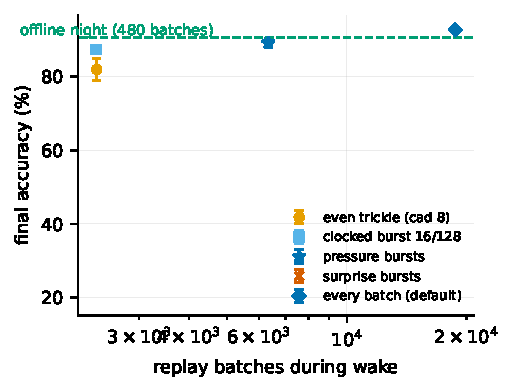
\includegraphics[width=.42\linewidth]{fig_timing.pdf}
\caption{\textbf{Replay timing at sparse budgets:} accuracy against the number of waking
replay events; trickles and clocked bursts fail alike, pressure-triggered bursts (star) keep
most of the accuracy at a third of the events, surprise triggering fires no events in this
regime.}
\label{fig:timing}
\end{figure}

\section{Isolation across replay batch sizes}
\label{app:isomargin}
Figure~\ref{fig:isomargin} extends Figure~\ref{fig:batch} to two-sample replay micro-batches
and shows, per batch size, the seed-paired margin of the full system over rotation with
unmasked replay (held-out split; six seeds at batches $2$, $4$ and $16$, three at $8$). From
$16$ down to $4$ the margin is $0.1$ $[-0.3,+0.5]$, $0.3$ $[-0.2,+0.6]$ and $0.3$
$[-0.5,+1.2]$: isolation costs nothing and buys nothing measurable in mean accuracy while the
rotation keeps the live coalition tolerant of unmasked replay. At batch $2$ the replay
gradient is too noisy for either system. The isolated one falls to $79.0\pm3.2$ (forgetting
$21.5\pm4.2$ against $6.4$ at batch $16$), with every seed between $75.5$ and $84.3$; the
unmasked one bifurcates, with three seeds finishing at $82.5$--$84.8$, slightly above their
isolated counterparts ($+0.3$, $+1.8$, $+8.1$), one at $58.2$ and two at chance ($9.9$).
Leaking replay onto the live coalition is therefore not a pure loss, since the surviving seeds
show that the extra plasticity can help, but it exposes a severe-failure mode (final accuracy
below $60\%$) that the isolated system did not show in six seeds. Six seeds without a severe
failure bound its frequency but do not prove the mode absent, and the masked system itself
destabilises at replay gain $10$ (Appendix~\ref{app:further}). The paired mean at batch $2$
($+24$ $[-0.2,+48.5]$) describes the unmasked failures, not a margin, and is kept out of the
ranges quoted in the main text.

\begin{figure}[h]
\centering
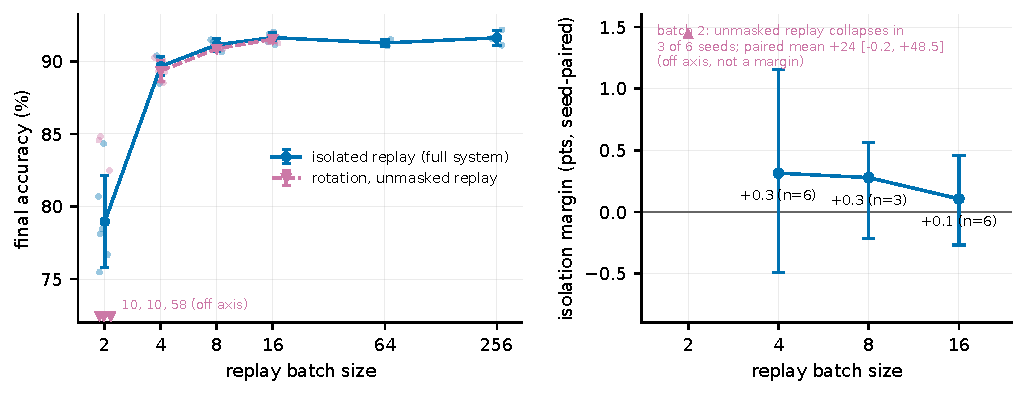
\includegraphics[width=.95\linewidth]{fig_isomargin.pdf}
\caption{\textbf{Isolation across replay batch sizes} (held-out split). \textbf{Left:}
split-MNIST accuracy against replay batch size for isolated replay (the full system) and for
rotation with unmasked replay, every seed shown; at batch $2$ no unmasked mean is drawn
because three of six seeds fail severely (values at the axis floor). \textbf{Right:} the
seed-paired margin of isolation with a $95\%$ bootstrap interval at the batch sizes where the
unmasked run does not collapse.}
\label{fig:isomargin}
\end{figure}

\section{A drive-referenced decay controller and depth}
\label{app:controller}
Every result in the main text runs the rule with a decay $\lambda$ tuned once per dataset
($10^{-3}$ on the image benchmarks). Split CIFAR-100 exposes what that constant hides: each
class receives a tenth of the supervision events while the decay acts on every synapse at
every step, so at the MNIST-tuned value the hidden weights follow the pure-decay trajectory
and the network lands at chance ($2.4\%$ i.i.d.\ against $20$--$23\%$ on a ten-class subset,
development-phase numbers). We replace the constant by a per-layer ratio controller,
\begin{equation}
\lambda_\ell=\min\!\Big(\lambda_{\max},\ \rho\,\mathrm{EMA}\big[u^\ell\big]\big/\big(\overline{|W^\ell|}+\epsilon\big)\Big),\qquad \rho=0.25,\ \lambda_{\max}=0.02,
\label{eq:controller}
\end{equation}
where $u^\ell$ is the mean magnitude of the post-optimiser, \emph{pre-decay} waking increment
of layer $\ell$ (the decay never feeds its own drive; EMA coefficient $0.02$ over unmasked
waking steps, $\epsilon=10^{-12}$), and $W^\ell$, $B^{\ell-1}$ share $\lambda_\ell$: the decay's
mean magnitude $\lambda_\ell\overline{|W^\ell|}$ is held at the fraction $\rho$ of the mean
data-driven update. $\rho$ is the only control target; $\lambda_{\max}$, the EMA coefficient
and $\epsilon$ are global safeguards never tuned per dataset. Isolation and rotation decide
\emph{where} and \emph{when} to consolidate, the controller \emph{how strongly}. The drive
estimate must see only unamplified waking updates: inflated targets and the offline night's
$3\times$-gain batches push the EMA to its clip and erase day learning.

\begin{table}[H]
\centering\footnotesize
\caption{\textbf{One dataset-independent ratio target replaces per-dataset decay tuning.}
Sequential / static accuracy under the tuned fixed decay ($10^{-3}$; $10^{-4}$ with $3\times$
targets as the CIFAR-100 rescue) and the controller \eqref{eq:controller} at $\rho=0.25$
everywhere. Full system in every cell, held-out split, three seeds (six on split-MNIST and in
the fixed-decay split CIFAR-10 cell); feature CIFAR feeds the images through a frozen
random-patch front-end (1024-D); CIFAR-100
numbers are floor-regime and reported for ordering only (BP+ER $6.8$ raw, $10.1$ with
features).}
\label{tab:controller}
\begin{tabular}{lcccc}
\toprule
& \multicolumn{2}{c}{fixed $\lambda$ (tuned)} & \multicolumn{2}{c}{controller} \\
& seq. & static & seq. & static \\
\midrule
split-MNIST & $91.6\pm0.3$ & $94.1\pm0.2$ & $90.6\pm0.6$ & $93.5\pm4.3$ \\
split CIFAR-10 & $28.4\pm0.8$ & $28.0\pm1.2$ & $26.2\pm1.1$ & $30.1\pm0.2$ \\
feature CIFAR-10 & $42.3\pm0.6$ & $42.4\pm1.1$ & $39.1\pm0.4$ & $43.6\pm0.6$ \\
split CIFAR-100 & $1.2\pm0.1$ & $1.0\pm0.1$ & $3.2\pm0.8$ & $4.1\pm0.6$ \\
\quad + features & $1.1\pm0.3$ & $1.1\pm0.2$ & $5.2\pm1.6$ & $6.4\pm0.6$ \\
\bottomrule
\end{tabular}
\end{table}

With the same $\rho$ on every dataset (Table~\ref{tab:controller}) the controller concedes
$1$--$3$ sequential points to the per-dataset tuned value and gains $1.2$--$5.3$ static
points on CIFAR-10, feature CIFAR-10 and both CIFAR-100 variants. On MNIST it gains $1.1$ on
the second held-out split ($95.2\pm0.4$) but one of six seeds collapsed on the first
($93.5\pm4.3$), so we claim no static gain there. On CIFAR-100 it lifts the system
$2.7$--$4.7\times$ over the manual rescue. The realised $\lambda_\ell$ spans $10^{-5}$ (MNIST
streams) to $3\times10^{-3}$ (raw CIFAR), so the per-dataset ladder was a signal-to-decay
ratio in disguise.

\paragraph{Depth.} Figure~\ref{fig:depth} varies the hidden depth. Under the tuned fixed
decay without skips the static axis dies at four hidden layers ($10.1\pm0.2\%$, chance) and
the sequential axis collapses at five ($26.3\pm20.2$); under the controller every cell stays
alive ($90.7\to88.9\to88.1$ sequential, $95.3\to94.8\to89.6$ static). The residual toll is
architectural. ResNet-style skip synapses restore the thick error path: for $\ell\ge3$ each
deep hidden layer receives a bypass, $z^\ell=W^\ell a^{\ell-1}+S^\ell a^{\ell-2}+b^\ell$, with
$S^\ell$ under the same Dale projection and a feedback twin
$B_S^{\ell}\in\mathbb{R}^{n_{\ell+2}\times n_\ell}$ that carries the bypass target's burst back
to its source, learned by the local product of the main text with the target layer's decay
$\lambda_\ell$ and replay-masked by the same rule two layers apart,
$M^{\ell}_{S,ij}=\mathbf{1}[\,j\notin\mathcal{A}^{\ell-2}(X)\ \lor\ i\notin\mathcal{A}^{\ell}(X)\,]$,
so that Propositions~\ref{prop:pre} and~\ref{prop:post} extend unchanged. The
five-hidden-layer system then reaches $91.0\pm0.3/95.8\pm0.3$ (six seeds) against the
two-layer default's $91.6/94.1$ and the two-layer controller's $90.6/93.5$. The bypass alone
also rescues the fixed decay ($90.4/93.5$ at depth five), so error-path attenuation is a
principal cause of the collapse (the fixed decay was not re-tuned per depth). BP+ER at the
same widths is depth-insensitive ($88.9\to87.9$) but forgets $2\times$ more.

\begin{figure}[h]
\centering
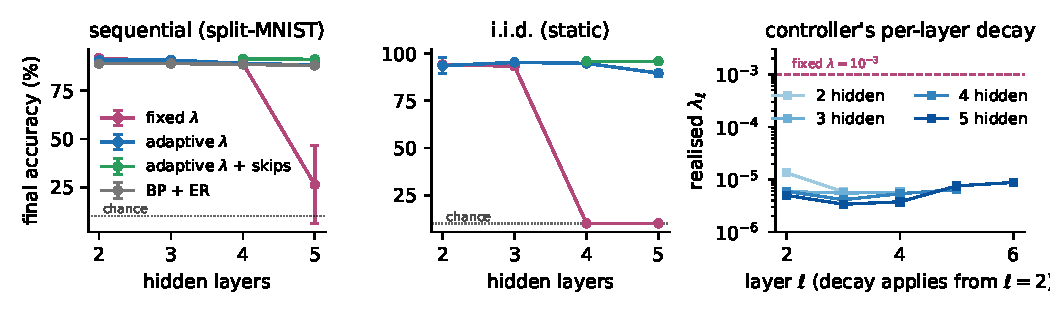
\includegraphics[width=.80\linewidth]{fig_depth.pdf}
\caption{\textbf{Depth.} Sequential (left) and static (middle) accuracy against hidden depth
(three seeds; six at the skip system's depth five): the fixed decay without skips collapses,
the controller degrades gracefully, controller $+$ skips hold the two-layer level. Right: the
controller's realised per-layer decay.}
\label{fig:depth}
\end{figure}

\section{Development-phase numbers and a second held-out split}
\label{app:val}
Configurations were selected on the official test splits (the development set) and frozen;
the comparisons in the main text re-train them on nine tenths of the training data and
evaluate on the held-out tenth, which took part in no selection. Table~\ref{tab:val} places
the development-set numbers beside the held-out ones and beside a second held-out tenth for
the headline rows (drawn with a different seed; the two tenths share $9\%$ of their samples,
so they are not disjoint test sets). Over the $87$ sequential configurations run under both
protocols, reported numbers sit $1.1$ points below the development numbers on average and
rank-correlate with them at Spearman $\rho=0.97$ (a robustness check, not a proof that
selection bias is absent); every ordering carried by the paper holds on both held-out splits,
with one magnitude that does not: the same-learner night, bimodal on the first split
($89.0\pm3.5$), reaches $91.5\pm0.5$ on the second and trails the full system by $0.3$ there.
The adaptive decay's static margin on MNIST is likewise split-dependent ($93.5\pm4.3$ with one
collapsed seed on the first split, $95.2\pm0.4$ on the second). Table~\ref{tab:accmatrix}
gives the per-task accuracy matrix of the headline configuration on the reported split.

\begin{table}[H]
\centering\small
\caption{\textbf{Development-set (official test split) numbers beside the held-out numbers and
a second held-out split.} Sequential accuracy, with the static axis on its own row
where the paper reports it; six seeds on the reported split, three on the development set and
on the second split. Lower blocks: single pass, and raw split CIFAR-10.}
\label{tab:val}
\begin{tabular}{@{}lccc@{}}
\toprule
& development set & held-out split 1 & held-out split 2 \\
\midrule
isolated replay $+$ rotation (default) & $92.7\pm0.3$ & $91.6\pm0.3$ & $91.8\pm0.4$ \\
\quad static & $94.7\pm0.3$ & $94.1\pm0.2$ & $94.1\pm0.6$ \\
bout-committed gate & $92.3\pm0.2$ & $91.8\pm0.3$ & $92.0\pm0.6$ \\
rotation alone (unmasked replay) & $92.1\pm0.5$ & $91.5\pm0.3$ & $91.8\pm0.6$ \\
\quad static & $94.7\pm0.1$ & $93.7\pm0.3$ & $93.7\pm0.3$ \\
silent mask (no rotation) & $88.8\pm0.8$ & $88.0\pm0.7$ & $88.6\pm1.3$ \\
unmasked interleaved replay & $87.0\pm1.1$ & $85.4\pm3.5$ & $80.0\pm14.1$ \\
BP $+$ ER & $89.3\pm0.8$ & $88.8\pm0.3$ & $88.5\pm0.7$ \\
offline night, same learner & $90.9\pm3.2$ & $89.0\pm3.5$ & $91.5\pm0.5$ \\
offline night, narrow learner & $90.7\pm0.4$ & $88.5\pm2.8$ & $89.3\pm0.6$ \\
adaptive $\lambda$ (drive) & $91.7\pm0.2$ & $90.6\pm0.6$ & $90.8\pm0.1$ \\
\quad static & $96.1\pm0.2$ & $93.5\pm4.3$ & $95.2\pm0.4$ \\
five hidden layers $+$ skips $+$ adaptive $\lambda$ & $91.5\pm0.4$ & $91.0\pm0.3$ & $91.1\pm0.3$ \\
\quad static & $96.2\pm0.3$ & $95.8\pm0.3$ & $95.7\pm0.1$ \\
no buffer & $19.6\pm0.0$ & $19.4\pm0.0$ & $19.5\pm0.0$ \\
random rotation & $90.8\pm1.3$ & $91.1\pm0.7$ & $90.7\pm0.5$ \\
replay confined to the readout & $27.3\pm15.1$ & $41.7\pm10.9$ & $38.1\pm4.9$ \\
mirror isolation & $77.9\pm1.6$ & $79.4\pm3.5$ & $79.2\pm2.4$ \\
soft rotation & $90.2\pm0.4$ & $89.9\pm0.7$ & $89.5\pm0.4$ \\
BP $+$ DER++ & $92.2\pm0.5$ & $91.5\pm0.5$ & $91.3\pm0.3$ \\
BP $+$ ER-ACE & $90.4\pm0.3$ & $90.2\pm0.4$ & $90.4\pm0.2$ \\
BP $+$ A-GEM & $73.6\pm4.2$ & $68.5\pm7.0$ & $70.4\pm4.1$ \\
BP $+$ \kwta{}, interleaved replay (same schedule) & $92.4\pm0.4$ & $91.7\pm0.4$ & --- \\
BP $+$ \kwta{}, isolated replay & $84.3\pm2.5$ & $84.7\pm2.6$ & --- \\
BP $+$ \kwta{}, interleaved replay $+$ rotation & $92.9\pm0.4$ & $92.2\pm0.3$ & --- \\
BP $+$ \kwta{}, isolated replay $+$ rotation & $92.9\pm0.2$ & $92.1\pm0.3$ & --- \\
\midrule
\multicolumn{4}{@{}l}{\emph{single pass (one epoch per task)}} \\
\quad isolated replay $+$ rotation & $91.8\pm0.4$ & $91.8\pm0.3$ & $91.8\pm0.1$ \\
\quad unmasked interleaved replay & $68.3\pm19.1$ & $83.0\pm14.9$ & $83.9\pm6.0$ \\
\quad offline night, same learner & $75.4\pm0.5$ & $76.9\pm3.4$ & $75.2\pm5.5$ \\
\quad BP $+$ ER & $90.1\pm0.7$ & $88.6\pm0.2$ & $88.2\pm0.9$ \\
\quad BP $+$ DER++ & --- & $90.1\pm0.7$ & $89.4\pm0.3$ \\
\midrule
\multicolumn{4}{@{}l}{\emph{split CIFAR-10 (raw)}} \\
\quad isolated replay $+$ rotation & $29.5\pm0.8$ & $28.4\pm0.8$ & $29.7\pm0.9$ \\
\quad offline night & $26.2\pm0.6$ & $25.1\pm2.7$ & $26.5\pm0.4$ \\
\quad BP $+$ ER & $25.1\pm1.5$ & $24.6\pm0.6$ & $25.8\pm0.8$ \\
\quad BP $+$ DER++ & $31.1\pm0.3$ & $30.7\pm0.8$ & $31.0\pm0.6$ \\
\quad BP $+$ ER-ACE & $31.7\pm0.8$ & $31.6\pm1.0$ & $31.7\pm0.8$ \\
\quad unmasked ER & $17.0\pm6.1$ & $14.6\pm4.6$ & $15.5\pm4.5$ \\
\quad no buffer & $16.4\pm0.2$ & $16.3\pm0.1$ & $16.6\pm0.0$ \\
\bottomrule
\end{tabular}
\end{table}

\begin{table}[H]
\centering\small
\caption{\textbf{Per-task accuracy matrix} of the headline configuration on split-MNIST
(held-out split, mean over six seeds): row $=$ after training task $i$, column $=$ accuracy on
task $j$. Forgetting $F$, the mean of the diagonal minus the last row over tasks $1$--$4$, is
$6.4\pm0.6$; the drop is concentrated on tasks $2$--$3$ and the first task is retained.}
\label{tab:accmatrix}
\begin{tabular}{lccccc}
\toprule
after task & T1 & T2 & T3 & T4 & T5 \\
\midrule
1 & $99.8$ & & & & \\
2 & $98.7$ & $97.2$ & & & \\
3 & $97.7$ & $92.7$ & $97.0$ & & \\
4 & $97.5$ & $89.6$ & $92.9$ & $97.5$ & \\
5 & $96.7$ & $88.1$ & $89.7$ & $91.5$ & $91.8$ \\
\bottomrule
\end{tabular}
\end{table}

\end{document}
